% Template of basic phisics experiment 基于 article template,在此基础上做修改
% 设定文章编码类型,正文字号为五号则 zihao=5,正文字号为小四则 zihao=-4
\documentclass[zihao=5, UTF8]{article}		


% 自定义宏定义
\def\N{\mathbb{N}}
\def\F{\mathbb{F}}
\def\Z{\mathbb{Z}}
\def\Q{\mathbb{Q}}
\def\R{\mathbb{R}}
\def\C{\mathbb{C}}
\def\T{\mathbb{T}}
\def\S{\mathbb{S}}
\def\A{\mathbb{A}}
\def\I{\mathscr{I}}
\def\d{\mathrm{d}}
\def\p{\partial}


% 物理实验报告所需的其它宏包
\usepackage{ulem}   % \uline 下划线支持

% 导入基本宏包
\usepackage[UTF8]{ctex}     % 设置文档为中文语言
\usepackage[colorlinks, linkcolor=blue, anchorcolor=blue, citecolor=blue, urlcolor=blue]{hyperref}  % 宏包:自动生成超链接 (此宏包与标题中的数学环境冲突)
% \usepackage{docmute}    % 宏包:子文件导入时自动去除导言区,用于主/子文件的写作方式,\include{./51单片机笔记}即可。注:启用此宏包会导致.tex文件capacity受限。
\usepackage{amsmath}    % 宏包:数学公式
\usepackage{mathrsfs}   % 宏包:提供更多数学符号
\usepackage{amssymb}    % 宏包:提供更多数学符号
\usepackage{pifont}     % 宏包:提供了特殊符号和字体
\usepackage{extarrows}  % 宏包:更多箭头符号

% 列表环境设置
\usepackage{enumitem}   % 宏包:列表环境设置
    \setlist[enumerate]{itemsep=0pt, parsep=0pt, topsep=0pt, partopsep=0pt, leftmargin=3.5em} 
    \setlist[itemize]{itemsep=0pt, parsep=0pt, topsep=0pt, partopsep=0pt, leftmargin=3.5em}
    \newlist{circledenum}{enumerate}{1} % 创建一个新的枚举环境  
    \setlist[circledenum,1]{  
        label=\protect\circled{\arabic*}, % 使用 \arabic* 来获取当前枚举计数器的值,并用 \circled 包装它  
        ref=\arabic*, % 如果需要引用列表项,这将决定引用格式(这里仍然使用数字)
        itemsep=0pt, parsep=0pt, topsep=0pt, partopsep=0pt, leftmargin=3.5em
    }  
% 文章页面 margin 设置
\usepackage[a4paper]{geometry}  % 宏包:文章页面 margin 设置
    \geometry{top=0.75in}
    \geometry{bottom=0.75in}
    \geometry{left=0.75in}
    \geometry{right=0.75in}   % 设置上下左右页边距
    \geometry{marginparwidth=1.75cm}    % 设置边注距离(注释、标记等)

% 自定义数学环境
\usepackage{amsthm} % 宏包:数学环境配置
% theorem-line 环境自定义
    \newtheoremstyle{MyLineTheoremStyle}% <name>
        {11pt}% <space above>
        {11pt}% <space below>
        {}% <body font> 使用默认正文字体
        {}% <indent amount>
        {\bfseries}% <theorem head font> 设置标题项为加粗
        {:}% <punctuation after theorem head>
        {.5em}% <space after theorem head>
        {\textbf{#1}\thmnumber{#2}\ \ (\,\textbf{#3}\,)}% 设置标题内容顺序
    \theoremstyle{MyLineTheoremStyle} % 应用自定义的定理样式
    \newtheorem{LineTheorem}{Theorem.\,}
% theorem-block 环境自定义
    \newtheoremstyle{MyBlockTheoremStyle}% <name>
        {11pt}% <space above>
        {11pt}% <space below>
        {}% <body font> 使用默认正文字体
        {}% <indent amount>
        {\bfseries}% <theorem head font> 设置标题项为加粗
        {:\\ \indent}% <punctuation after theorem head>
        {.5em}% <space after theorem head>
        {\textbf{#1}\thmnumber{#2}\ \ (\,\textbf{#3}\,)}% 设置标题内容顺序
    \theoremstyle{MyBlockTheoremStyle} % 应用自定义的定理样式
    \newtheorem{BlockTheorem}[LineTheorem]{Theorem.\,} % 使用 LineTheorem 的计数器
% definition 环境自定义
    \newtheoremstyle{MySubsubsectionStyle}% <name>
        {11pt}% <space above>
        {11pt}% <space below>
        {}% <body font> 使用默认正文字体
        {}% <indent amount>
        {\bfseries}% <theorem head font> 设置标题项为加粗
        {:\\ \indent}% <punctuation after theorem head>
        {0pt}% <space after theorem head>
        {\textbf{#3}}% 设置标题内容顺序
    \theoremstyle{MySubsubsectionStyle} % 应用自定义的定理样式
    \newtheorem{definition}{}


% 有色文本框及其设置
\usepackage[dvipsnames,svgnames]{xcolor}    %设置插入的文本框颜色
\usepackage[strict]{changepage}     % 提供一个 adjustwidth 环境
\usepackage{framed}     % 实现方框效果
    \definecolor{graybox_color}{rgb}{0.95,0.95,0.96} % 文本框颜色。修改此行中的 rgb 数值即可改变方框纹颜色,具体颜色的rgb数值可以在网站https://colordrop.io/ 中获得。(截止目前的尝试还没有成功过,感觉单位不一样)(找到喜欢的颜色,点击下方的小眼睛,找到rgb值,复制修改即可)
    \newenvironment{graybox}{%
    \def\FrameCommand{%
    \hspace{1pt}%
    {\color{gray}\small \vrule width 2pt}%
    {\color{graybox_color}\vrule width 4pt}%
    \colorbox{graybox_color}%
    }%
    \MakeFramed{\advance\hsize-\width\FrameRestore}%
    \noindent\hspace{-4.55pt}% disable indenting first paragraph
    \begin{adjustwidth}{}{7pt}%
    \vspace{2pt}\vspace{2pt}%
    }
    {%
    \vspace{2pt}\end{adjustwidth}\endMakeFramed%
    }

% 各级标题自定义设置
\usepackage{titlesec}   
    % section标题自定义设置 
    \titleformat{\section}[hang]{\normalfont\huge\bfseries\centering}{第\,\thesection\,部分}{20pt}{}
    % subsection标题自定义设置 
    \titleformat{\subsection}[hang]{\normalfont\Large\bfseries}{\,\thesubsection\,}{8pt}{}
    % subsubsection标题自定义设置
    \titleformat{\subsubsection}[hang]{\normalfont\large\bfseries}{\,\thesubsubsection\,}{6pt}{}

% 外源代码插入设置
\usepackage{matlab-prettifier}
    \lstset{
        style=Matlab-editor,  % 继承matlab代码颜色等
    }
\usepackage[most]{tcolorbox} % 引入tcolorbox包 
\usepackage{listings} % 引入listings包
    \tcbuselibrary{listings, skins, breakable}
    \lstdefinestyle{matlabstyle}{
        language=Matlab,
        basicstyle=\small,
        breakatwhitespace=false,
        breaklines=true,
        captionpos=b,
        keepspaces=true,
        numbers=left,
        numbersep=15pt,
        showspaces=false,
        showstringspaces=false,
        showtabs=false,
        tabsize=2
    }
    \newtcblisting{matlablisting}{
        arc=0pt,
        top=0pt,
        bottom=0pt,
        left=1mm,
        listing only,
        listing style=matlabstyle,
        breakable,
        colback=white   % 选一个合适的颜色
    }
    % 自定义Verilog代码样式
\lstdefinelanguage{Verilog}{
    keywords=[1]{module, input, output, wire, assign, endmodule},
    keywords=[2]{always, if, else, case, endcase, begin, end},
    sensitive=true,
    morecomment=[l]{//},
    morecomment=[s]{/*}{*/},
    morestring=[b]",
}

\lstset{
    language=Verilog,
    basicstyle=\ttfamily\small,
    keywordstyle=[1]\color{blue},
    keywordstyle=[2]\color{purple},
    commentstyle=\color{gray},
    stringstyle=\color{orange},
    showstringspaces=false,
    numbers=left,
    numberstyle=\tiny\color{gray},
    stepnumber=1,
    numbersep=5pt,
    frame=single,
    tabsize=4,
    breaklines=true,
    backgroundcolor=\color{lightgray!10}
}

% table 支持
\usepackage{booktabs}   % 宏包:三线表
\usepackage{tabularray} % 宏包:表格排版
\usepackage{longtable}  % 宏包:长表格
\usepackage{tabularx}  % 宏包:宽表格
\usepackage{multirow}  % 宏包:表格中一格显示多个项目

% figure 设置
\usepackage{graphicx}  % 支持 jpg, png, eps, pdf 图片 
\usepackage{svg}       % 支持 svg 图片
    \svgsetup{
        % 指向 inkscape.exe 的路径
        inkscapeexe = C:/aa_MySame/inkscape/bin/inkscape.exe, 
        % 一定程度上修复导入后图片文字溢出几何图形的问题
        inkscapelatex = false                 
    }


% 图表进阶设置
\usepackage{float}     % 图表位置浮动设置 
\usepackage{caption}    % 图注、表注
    \captionsetup[figure]{name=图}  
    \captionsetup[table]{name=表}
    \captionsetup{labelfont=bf, font=small}

% 文章默认字体设置
    \usepackage{fontspec}   % 宏包:字体设置
       \setmainfont{SimSun}    % 设置中文字体为宋体字体
      \setCJKmainfont[AutoFakeBold=3]{SimSun} % 设置加粗字体为 SimSun 族,AutoFakeBold 可以调整字体粗细^     \setmainfont{Times New Roman} % 设置英文字体为Times New Roman

% 代码环境设置
\usepackage{minted}


% 其它设置
    % equation 公式编号设置
        \makeatletter  
        \renewcommand{\theequation}{\thesection.\arabic{equation}}  
        \makeatother
    % 脚注设置
        \renewcommand\thefootnote{\ding{\numexpr171+\value{footnote}}}
    % 参考文献引用设置
        \bibliographystyle{unsrt}   % 设置参考文献引用格式为unsrt
        \newcommand{\upcite}[1]{\textsuperscript{\cite{#1}}}     % 自定义上角标式引用
    % 文章序言设置
        \newcommand{\cnabstractname}{序言}
        \newenvironment{cnabstract}{%
            \par\Large
            \noindent\mbox{}\hfill{\bfseries \cnabstractname}\hfill\mbox{}\par
            \vskip 2.5ex
            }{\par\vskip 2.5ex}


% 页眉页脚设置
\usepackage{fancyhdr}   %宏包:页眉页脚设置
    \pagestyle{fancy}
    \fancyhf{}
    \cfoot{\thepage}
    \renewcommand\headrulewidth{1pt}
    \renewcommand\footrulewidth{0pt}
    %\rhead{\bfseries 分组序号: YK04-2}    
    \chead{《数字电路》实验报告,\ 韩初晓,\ 2023K8009908002}
    \lhead{2024.11.2}

% 文档信息设置
%\title{这里是标题\\The Title of the Report}
%\author{丁毅\\ \footnotesize 中国科学院大学,北京 100049\\ Yi Ding \\ %\footnotesize University of Chinese Academy of Sciences, Beijing %100049, China}
%\date{\footnotesize 2024.8 -- 2025.1}

% 开始编辑文章

\begin{document}
%\noindent\begin{flushright}
%   \zihao{2}{分组序号: YK04-2}
%\end{flushright}

\setCJKfamilyfont{boldsong}[AutoFakeBold = {2.17}]{SimSun}
\newcommand*{\boldsong}{\CJKfamily{boldsong}}


\begin{center}\large
    \noindent{\Huge\bfseries\boldsong《数字电路》实验报告 }
    \\\vspace{0.4cm}
    \noindent\textit{
        \textbf{\boldsong 实验名称:}\uline{\hspace{1.7cm} 比较器与超前进位加法器\hspace{1.7cm}}\hspace{0.4cm} 
        指导教师:\uline{\hspace{1.0cm}王珎,范志华\hspace{1.0cm}}}
    \\\vspace{0.1cm}
    \noindent\textit{
        姓名:\uline{\,\,\,韩初晓\,\,\,}\hspace{0.2cm}
        学号:\uline{\,\,\,{\upshape 2023K8009908002}\,\,\,}\hspace{0.2cm}
        专业:\uline{\,\,\,计算机科学与技术\,\,\,}\hspace{0.2cm}
        班级:\uline{\,\,\,\upshape{2306}\,\,\,}}
    \\\vspace{0.1cm}
    \noindent\textit{
        实验日期:\uline{\,\,{\upshape 2024.10.17}\,\,}\hspace{0.2cm}
        实验地点:\uline{\,\,\,教学楼{\upshape224}\,\,\,}\hspace{0.2cm}
        是否调课/补课:\uline{\hspace{0.5cm}否\hspace{0.5cm}}\hspace{0.2cm}
        成绩:\uline{\hspace{2cm}}}
\end{center}
% \vspace{-0.2cm}
\noindent\rule{\textwidth}{0.1em}   % 分割线

% 控制目录不换页
\vspace{1cm}
\setcounter{tocdepth}{2}  % 目录深度为 2(不显示 subsubsection)
\noindent\begin{minipage}{\textwidth}\centering
\tableofcontents\thispagestyle{fancy}   % 显示页码、页眉等   
\end{minipage}  
\newpage

\section{实验目的}\thispagestyle{fancy}
\begin{enumerate}
    \item 熟悉 Verilog 编程与调试方法。
    \item 熟悉简单比较器的工作原理。
    \item 通过简单模块例化、连线实现复杂的数字电路。
\end{enumerate}

\subsection{实验环境}
\begin{itemize}
    \item Vivado 2017.4 开发工具
    \item FPGA 开发平台(根据手册中的默认设置进行选择)
\end{itemize}


\section{实验内容}

\subsection{实验一:实现四位比较器}
\subsubsection{原理说明}
四位比较器用于比较两个四位二进制数 $A$ 和 $B$ 的大小关系。模块通过输入信号 \texttt{in\_A\_G\_B}、\texttt{in\_A\_E\_B}、\texttt{in\_A\_L\_B} 控制是否进行比较或直接传递输入值作为输出。比较的结果通过输出信号 \texttt{out\_A\_G\_B}、\texttt{out\_A\_E\_B} 和 \texttt{out\_A\_L\_B} 表示,即当 $A > B$ 时 \texttt{out\_A\_G\_B} 为 1;当 $A = B$ 时 \texttt{out\_A\_E\_B} 为 1;当 $A < B$ 时 \texttt{out\_A\_L\_B} 为 1。控制信号用于决定模块行为,具体如下:
\begin{itemize}
    \item \texttt{in\_A\_E\_B}:根据 $A$ 和 $B$ 的大小关系输出比较结果。
    \item \texttt{in\_A\_G\_B} 和 \texttt{in\_A\_L\_B}:直接将输入信号传递至输出,不进行比较。
\end{itemize}

\subsubsection{接口定义}
\begin{itemize}
    \item 输入信号:
    \begin{itemize}
        \item \texttt{A[3:0]}:四位二进制数,用于比较的第一个数。
        \item \texttt{B[3:0]}:四位二进制数,用于比较的第二个数。
        \item \texttt{in\_A\_G\_B}:输入控制信号,指示是否直接传递 $A > B$ 的结果。
        \item \texttt{in\_A\_E\_B}:输入控制信号,指示是否直接传递 $A = B$ 的结果。
        \item \texttt{in\_A\_L\_B}:输入控制信号,指示是否直接传递 $A < B$ 的结果。
    \end{itemize}
    \item 输出信号:
    \begin{itemize}
        \item \texttt{out\_A\_G\_B}:表示比较结果,当 $A > B$ 时为 1。
        \item \texttt{out\_A\_E\_B}:表示比较结果,当 $A = B$ 时为 1。
        \item \texttt{out\_A\_L\_B}:表示比较结果,当 $A < B$ 时为 1。
    \end{itemize}
\end{itemize}

\subsubsection{调试过程及结果}
在 \texttt{comparator\_4} 模块中,通过编写 Testbench 对其进行仿真测试,验证了模块在不同输入条件下的正确性。仿真波形展示了输入信号 $A$、$B$ 以及控制信号的变化情况,输出 \texttt{out\_A\_G\_B}、\texttt{out\_A\_E\_B} 和 \texttt{out\_A\_L\_B} 依照输入正确反映了比较结果,仿真结果如下:
\begin{figure}[htbp]
    \centering
    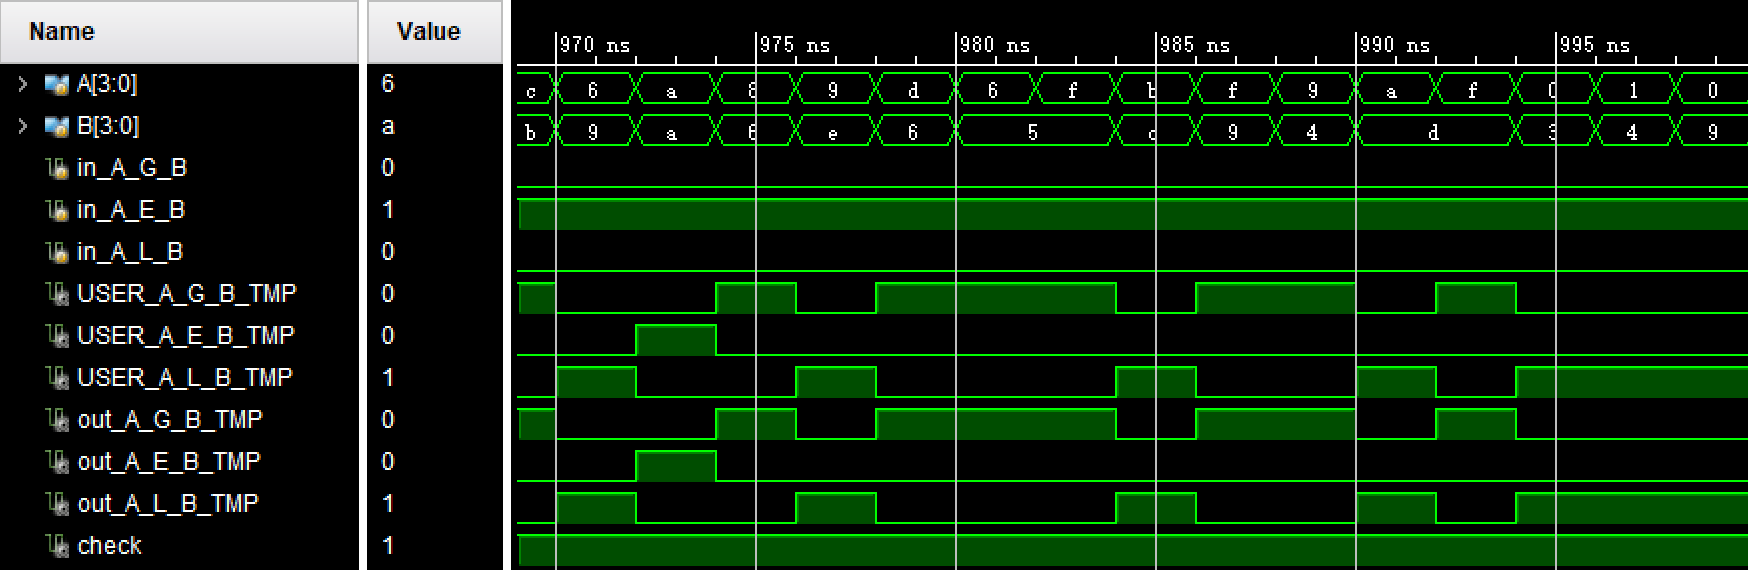
\includegraphics[width=\textwidth]{comparator_4.png} % 图片路径和大小
    \caption{comparator\_4 模块的测试结果}
    \label{fig:comparator_4模块的测试结果}
\end{figure}


\subsection{实验二:实现十六位比较器}
\subsubsection{原理说明}
十六位比较器模块 \texttt{comparator\_16} 用于比较两个十六位二进制数 $A$ 和 $B$ 的大小关系。该模块将十六位数 $A$ 和 $B$ 分为 4 个 4 位段,并使用四个 \texttt{comparator\_4} 模块逐级比较每 4 位段的大小关系。通过链式结构实现逐级比较,最终的比较结果输出至 \texttt{out\_A\_G\_B}、\texttt{out\_A\_L\_B} 和 \texttt{out\_A\_E\_B}。模块工作原理如下:

1. 首先比较最高位段 $A[15:12]$ 和 $B[15:12]$ 的大小,将结果传递至下一比较器。
2. 接着比较次高位段 $A[11:8]$ 和 $B[11:8]$,基于前一级比较结果继续传递比较结果。
3. 同理,比较 $A[7:4]$ 与 $B[7:4]$,以及最低位段 $A[3:0]$ 和 $B[3:0]$。
4. 最终,将最低位段的比较结果传递给输出端,完成对十六位二进制数的整体比较。

\subsubsection{接口定义}
\begin{itemize}
    \item 输入信号:
    \begin{itemize}
        \item \texttt{A[15:0]}:十六位二进制数,用于比较的第一个数。
        \item \texttt{B[15:0]}:十六位二进制数,用于比较的第二个数。
        \item \texttt{in\_A\_G\_B}:输入控制信号,指示是否直接传递 $A > B$ 的结果。
        \item \texttt{in\_A\_L\_B}:输入控制信号,指示是否直接传递 $A < B$ 的结果。
        \item \texttt{in\_A\_E\_B}:输入控制信号,指示是否直接传递 $A = B$ 的结果。
    \end{itemize}
    \item 输出信号:
    \begin{itemize}
        \item \texttt{out\_A\_G\_B}:表示比较结果,当 $A > B$ 时为 1。
        \item \texttt{out\_A\_E\_B}:表示比较结果,当 $A = B$ 时为 1。
        \item \texttt{out\_A\_L\_B}:表示比较结果,当 $A < B$ 时为 1。
    \end{itemize}
\end{itemize}

\subsubsection{调试过程及结果}
在 \texttt{comparator\_16} 模块中,通过编写 Testbench 对其进行仿真测试,验证了模块在不同输入条件下的正确性。仿真波形展示了输入信号 $A$、$B$ 以及中间信号 \texttt{result4}、\texttt{result3}、\texttt{result2} 的变化情况,输出 \texttt{out\_A\_G\_B}、\texttt{out\_A\_E\_B} 和 \texttt{out\_A\_L\_B} 依照输入正确反映了比较结果,仿真结果如下:
\begin{figure}[htbp]
    \centering
    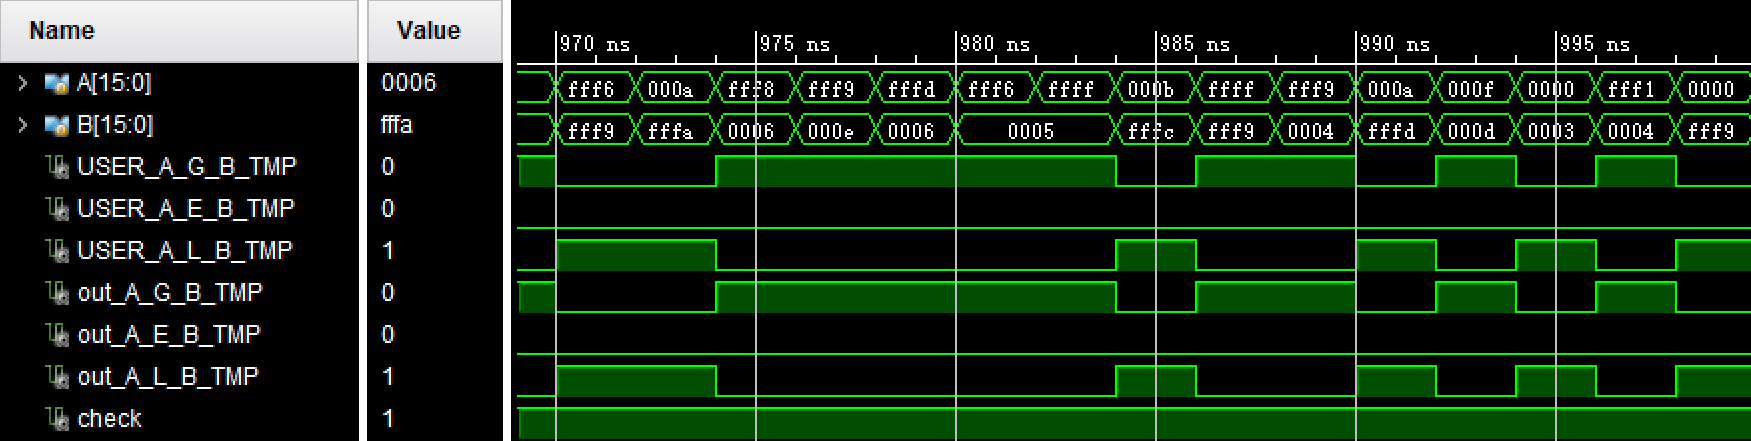
\includegraphics[width=\textwidth]{comparator_16.png} % 图片路径和大小
    \caption{comparator\_16 模块的测试结果}
    \label{fig:comparator_16模块的测试结果}
\end{figure}

\subsection{实验三:实现四位加法器}
\subsubsection{原理说明}
四位加法器模块 \texttt{adder\_4} 通过输入两个 4 位二进制数 \texttt{num\_1} 和 \texttt{num\_2},以及进位输入 \texttt{cin},计算出 4 位和 \texttt{result} 和进位输出 \texttt{cout}。模块使用生成信号($g$)和传播信号($p$)进行加法运算,以优化进位的生成过程。

具体原理如下:
1. 计算生成信号 $g[i] = \texttt{num\_1[i]} \& \texttt{num\_2[i]}$ 和传播信号 $p[i] = \texttt{num\_1[i]} | \texttt{num\_2[i]}$。
2. 通过组合逻辑生成每一位的进位 $c[i]$,最终得到 \texttt{cout}。
3. 通过表达式 \texttt{result = ~g \& p \textasciicircum c[3:0]} 得到四位加法结果 \texttt{result}。

\subsubsection{接口定义}
\begin{itemize}
    \item 输入信号:
    \begin{itemize}
        \item \texttt{cin}:输入进位信号,用于处理来自前一级的进位。
        \item \texttt{num\_1[3:0]}:四位二进制数,第一个加数。
        \item \texttt{num\_2[3:0]}:四位二进制数,第二个加数。
    \end{itemize}
    \item 输出信号:
    \begin{itemize}
        \item \texttt{result[3:0]}:四位加法运算的结果。
        \item \texttt{cout}:加法运算的进位输出信号,表示最高位的进位。
    \end{itemize}
\end{itemize}

\subsubsection{调试过程及结果}
在 \texttt{adder\_4} 模块中,通过编写 Testbench 对其进行仿真测试,验证模块在不同输入条件下的正确性。仿真波形展示了输入信号 \texttt{num\_1}、\texttt{num\_2}、\texttt{cin} 的变化情况,输出 \texttt{result} 和 \texttt{cout} 正确反映了加法结果和进位输出,仿真结果如下:
\begin{figure}[htbp]
    \centering
    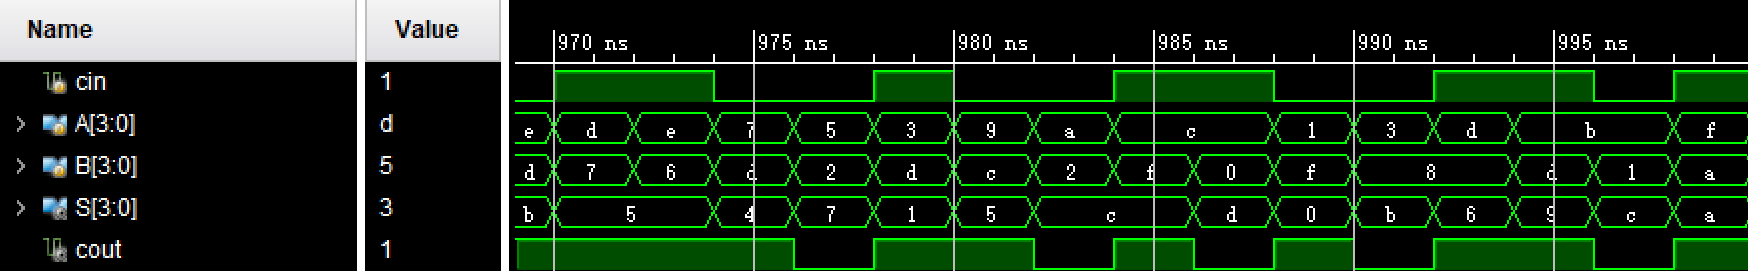
\includegraphics[width=\textwidth]{adder_4.png} % 图片路径和大小
    \caption{adder\_4 模块的测试结果}
    \label{fig:adder_4模块的测试结果}
\end{figure}

\subsection{实验四:实现三十二位超前进位加法器}
\subsubsection{原理说明}
三十二位超前进位加法器模块 \texttt{add\_32} 通过分组加法与进位生成模块实现快速加法运算。该模块由多个子模块构成,包括 4 位加法器、进位生成模块、生成与传播信号计算模块等,以提高计算速度。

具体原理如下:
1. 将 32 位输入数 \texttt{num\_1} 和 \texttt{num\_2} 分为 8 个 4 位子块。
2. 通过连接上层的单元实现($g$)和($p$)信号的生成,从而快速生成进位。
3. 最终输出 32 位加法结果 \texttt{result} 和进位输出 \texttt{cout}。

\begin{figure}[htbp]
    \centering
    % 这里填写你的图片路径
    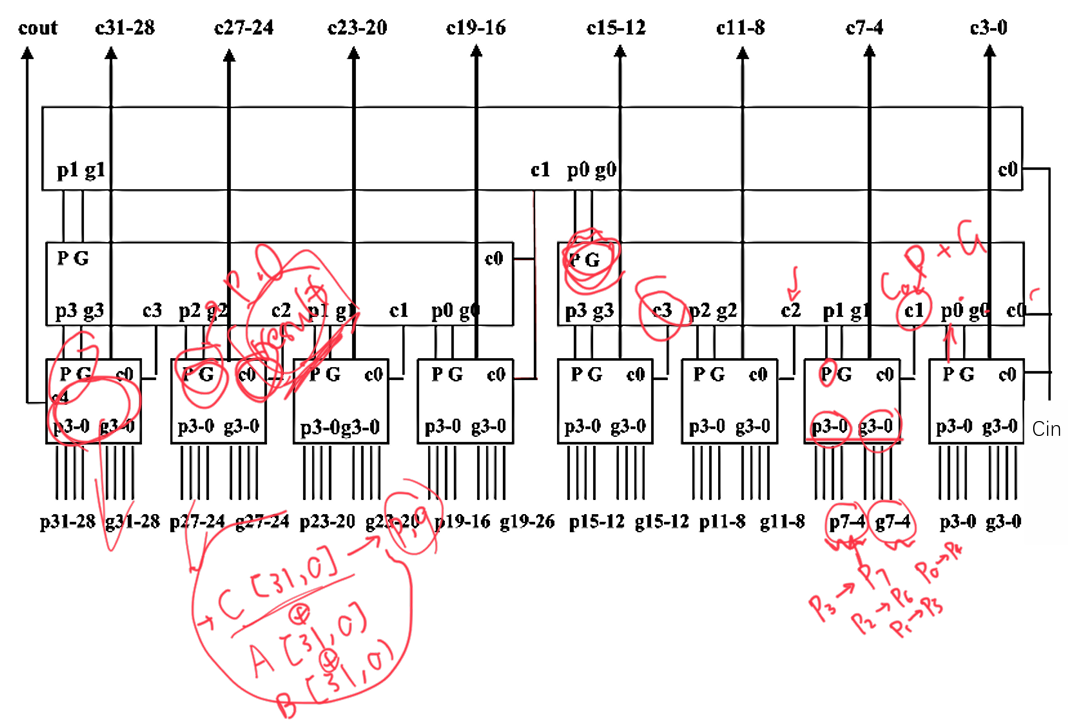
\includegraphics[width=0.8\textwidth]{三十二位超前进位加法器.png}
    \caption{32位超前进位加法器的示意图}
    \label{fig:cla32}
\end{figure}

\subsubsection{接口定义}
\begin{itemize}
    \item 输入信号:
    \begin{itemize}
        \item \texttt{cin}:输入进位信号,用于处理来自前一级的进位。
        \item \texttt{num\_1[31:0]}:32 位二进制数,第一个加数。
        \item \texttt{num\_2[31:0]}:32 位二进制数,第二个加数。
    \end{itemize}
    \item 输出信号:
    \begin{itemize}
        \item \texttt{result[31:0]}:32 位加法运算的结果。
        \item \texttt{cout}:加法运算的进位输出信号,表示最高位的进位。
    \end{itemize}
\end{itemize}

\subsubsection{调试过程及结果}
在 \texttt{add\_32} 模块中,通过编写 Testbench 对其进行仿真测试,验证模块在不同输入条件下的正确性。仿真波形展示了输入信号 \texttt{num\_1}、\texttt{num\_2}、\texttt{cin} 的变化情况,输出 \texttt{result} 和 \texttt{cout} 正确反映了加法结果和进位输出,仿真结果如下:
\begin{figure}[htbp]
    \centering
    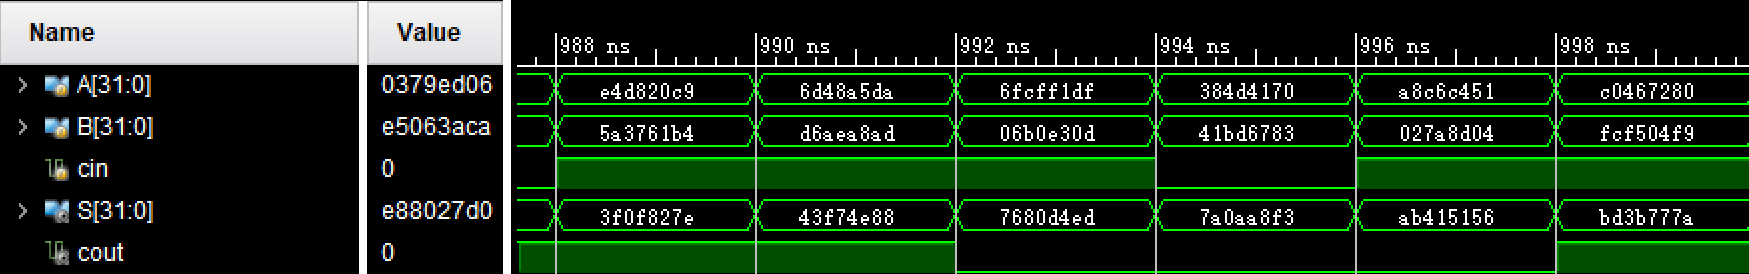
\includegraphics[width=\textwidth]{add_32.png} % 图片路径和大小
    \caption{add\_32 模块的测试结果}
    \label{fig:add_32模块的测试结果}
\end{figure}




\section{实验总结}

在本实验中,我通过 Verilog 实现了四个数字电路模块:四位比较器,十六位比较器,四位超前进位加法器和三十二位超前进位加法器。

通过四位和十六位比较器的实现,我更深入地理解了模块在 Verilog 中的实现方法,以及模块之间的连接方式。

在实现四位加法器时,我体会到了代码书写形式不同对实际电路生成结果的影响。例如,表示进位 \(c\) 的两个等价的逻辑表达式很可能一个生成出来的电路是串行的,而另一个生成出来的电路则是并行的。如果想要实际生成的电路计算效率高,在书写代码时就应当加以注意。

此外,在实现三十二位超前进位加法器的过程中,我经历了多次试错,最终将四位加法器拆成了 \texttt{pg\_generator}, \texttt{CLU} 等模块,并按实际工作的输入输出顺序连接起来,才使得模块正常工作。这启发我在书写代码时应当时刻考虑电路真正的工作过程,否则设计出的电路很可能会产生逻辑错误。

\section{源代码}

\subsection{实验一:实现四位比较器}

\begin{lstlisting}[language=Verilog]

module comparator_4(
    input [3:0] A,
    input [3:0] B,
    output reg out_A_G_B,
    output reg out_A_E_B,
    output reg out_A_L_B,
    input in_A_G_B,
    input in_A_E_B,
    input in_A_L_B
  );

    wire [2:0] control;
    assign control = {in_A_G_B, in_A_L_B, in_A_E_B};

    always @(*) begin
      if (control == 3'b001) begin
        if (A > B) begin
          out_A_G_B = 1'b1;
          out_A_L_B = 1'b0;
          out_A_E_B = 1'b0;
        end
        else if (A < B) begin
          out_A_G_B = 1'b0;
          out_A_L_B = 1'b1;
          out_A_E_B = 1'b0;
        end
        else if (A == B) begin
          out_A_G_B = 1'b0;
          out_A_L_B = 1'b0;
          out_A_E_B = 1'b1;
        end
      end
      else if (control == 3'b100) begin
        out_A_G_B = in_A_G_B;
        out_A_L_B = in_A_L_B;
        out_A_E_B = in_A_E_B;
      end
      else if (control == 3'b010) begin 
        out_A_G_B = in_A_G_B;
        out_A_L_B = in_A_L_B;
        out_A_E_B = in_A_E_B;
      end
    end
endmodule

\end{lstlisting}

\subsection{实验二:实现十六位比较器}
\begin{lstlisting}[language=Verilog]

module comparator_16(
    input [15:0] A,
    input [15:0] B,
    input in_A_G_B,
    input in_A_L_B,
    input in_A_E_B,
    output out_A_G_B,
    output out_A_L_B,
    output out_A_E_B
    );

    wire [2:0] result4;
    wire [2:0] result3;
    wire [2:0] result2;

    comparator_4 comparator_4_4(
    .A(A[15:12]),
    .B(B[15:12]),
    .in_A_G_B(in_A_G_B),
    .in_A_L_B(in_A_L_B),
    .in_A_E_B(in_A_E_B),
    .out_A_G_B(result4[2]),
    .out_A_L_B(result4[1]),
    .out_A_E_B(result4[0])
    );

    comparator_4 comparator_4_3(
    .A(A[11:8]),
    .B(B[11:8]),
    .in_A_G_B(result4[2]),
    .in_A_L_B(result4[1]),
    .in_A_E_B(result4[0]),
    .out_A_G_B(result3[2]),
    .out_A_L_B(result3[1]),
    .out_A_E_B(result3[0])
    );

    comparator_4 comparator_4_2(
    .A(A[7:4]),
    .B(B[7:4]),
    .in_A_G_B(result3[2]),
    .in_A_L_B(result3[1]),
    .in_A_E_B(result3[0]),
    .out_A_G_B(result2[2]),
    .out_A_L_B(result2[1]),
    .out_A_E_B(result2[0])
    );

    comparator_4 comparator_4_1(
    .A(A[3:0]),
    .B(B[3:0]),
    .in_A_G_B(result2[2]),
    .in_A_L_B(result2[1]),
    .in_A_E_B(result2[0]),
    .out_A_G_B(out_A_G_B),
    .out_A_L_B(out_A_L_B),
    .out_A_E_B(out_A_E_B)
    );
endmodule

\end{lstlisting}

\subsection{实验三:实现四位加法器}
\begin{lstlisting}[language=Verilog]

module adder_4(
    input cin,
    input [3:0] num_1,
    input [3:0] num_2,
    output [3:0] result,
    output cout
    );

    wire [3:0] p;
    wire [3:0] g;
    wire [4:0] c;

    assign p = num_1 | num_2;
    assign g = num_1 & num_2;
    assign c[0] = cin; 
  	assign c[1]=g[0]|cin&p[0];
  	assign c[2]=g[1]|g[0]&p[1]|cin&p[1]&p[0];
  	assign c[3]=g[2]|g[1]&p[2]|g[0]&p[2]&p[1]|cin&p[2]&p[1]&p[0];
  	assign c[4]=g[3]|g[2]&p[3]|g[1]&p[3]&p[2]|g[0]&p[3]&p[2]&p[1]|cin&p[3]&p[2]&p[1]&p[0];
    
    assign result = ~ g & p ^ c[3:0];
    assign cout = c[4];

endmodule

\end{lstlisting}

\subsection{实验四:实现三十二位超前进位加法器}

\begin{lstlisting}[language=Verilog]

module adder_component_clu(
  input [3:0] g,
  input [3:0] p,
  input ci,
  output [3:0] c
);
	assign c[0]=g[0]|ci&p[0];
	assign c[1]=g[1]|g[0]&p[1]|ci&p[1]&p[0];
	assign c[2]=g[2]|g[1]&p[2]|g[0]&p[2]&p[1]|ci&p[2]&p[1]&p[0];
	assign c[3]=g[3]|g[2]&p[3]|g[1]&p[3]&p[2]|g[0]&p[3]&p[2]&p[1]|ci&p[3]&p[2]&p[1]&p[0];

endmodule

module adder_component_tu(
  input [3:0] g,
  input [3:0] p,
  output [3:0] t
);
  assign t = ~g & p;

endmodule

module adder_component_pg_generator(
  input a,
  input b,
  
  output g,
  output p
);
  assign g = a & b;
  assign p = a | b;

endmodule

module adder_4m1(
    input cin,
    input [3:0] num_1,
    input [3:0] num_2,
    output [3:0] result,
    output [3:0] c
    //output pm,
    //output gm
    );

    wire [3:0] p_cla;
    wire [3:0] g_cla;
    wire [3:0] t_cla;
    wire [3:0] co_clu;

    adder_component_pg_generator PG0 (
    .a(num_1[0]),
    .b(num_2[0]),
    .g(g_cla[0]),
    .p(p_cla[0])
    );

    adder_component_pg_generator PG1 (
      .a(num_1[1]),
      .b(num_2[1]),
      .g(g_cla[1]),
      .p(p_cla[1])
    );

    adder_component_pg_generator PG2 (
      .a(num_1[2]),
      .b(num_2[2]),
      .g(g_cla[2]),
      .p(p_cla[2])
    );

    adder_component_pg_generator PG3 (
      .a(num_1[3]),
      .b(num_2[3]),
      .g(g_cla[3]),
      .p(p_cla[3])
    );

    adder_component_tu TU(
      .g(g_cla),
      .p(p_cla),
      .t(t_cla)
    );

    adder_component_clu CLU(
      .p(p_cla),
      .g(g_cla),
      .ci(cin),
      .c(co_clu)
    );

    assign result[0] = t_cla[0] ^ cin;
    assign result[1] = t_cla[1] ^ co_clu[0];
    assign result[2] = t_cla[2] ^ co_clu[1];
    assign result[3] = t_cla[3] ^ co_clu[2];
    assign c = {co_clu[2], co_clu[1], co_clu[0], cin};
   // assign pm = g_cla[3] | (p_cla[3] & g_cla[2]) | (p_cla[3] & p_cla[2] & g_cla[1]) | (p_cla[3] & p_cla[2] & p_cla[1] & g_cla[0]);
   // assign gm = p_cla[3] & p_cla[2] & p_cla[1] & p_cla[0];
endmodule

module pggenerator(
    input cin,
    input [3:0] p,
    input [3:0] g,
    output pm,
    output gm,
    output [3:0] c
    );

    wire [3:0] co_clu;

    adder_component_clu CLU(
      .p(p),
      .g(g),
      .ci(cin),
      .c(co_clu)
    );

    assign c[0] = cin;
    assign c[1] = co_clu[0];
    assign c[2] = co_clu[1];
    assign c[3] = co_clu[2];
    assign pm = g[3] | (p[3] & g[2]) | (p[3] & p[2] & g[1]) | (p[3] & p[2] & p[1] & g[0]);
    assign gm = p[3] & p[2] & p[1] & p[0];
endmodule

module cla_component_pgm_generator(
  input [3:0] num_1,
  input [3:0] num_2,

  output pm,
  output gm
);

    wire [3:0] g;
    wire [3:0] p;

      adder_component_pg_generator PG0 (
    .a(num_1[0]),
    .b(num_2[0]),
    .g(g[0]),
    .p(p[0])
    );

    adder_component_pg_generator PG1 (
      .a(num_1[1]),
      .b(num_2[1]),
      .g(g[1]),
      .p(p[1])
    );

    adder_component_pg_generator PG2 (
      .a(num_1[2]),
      .b(num_2[2]),
      .g(g[2]),
      .p(p[2])
    );

    adder_component_pg_generator PG3 (
      .a(num_1[3]),
      .b(num_2[3]),
      .g(g[3]),
      .p(p[3])
    );

  assign gm=g[3]|g[2]&p[3]|g[1]&p[3]&p[2]|g[0]&p[3]&p[2]&p[1];
	assign pm=p[3]&p[2]&p[1]&p[0];

endmodule

module cla_generate_from_pg (
  input [3:0] g,
	input [3:0] p,
	
	output gm,
	output pm
);
	
	assign gm=g[3]|g[2]&p[3]|g[1]&p[3]&p[2]|g[0]&p[3]&p[2]&p[1];
	assign pm=p[3]&p[2]&p[1]&p[0];
	
endmodule

module add_32(
      input [31:0] num_1,
      input [31:0] num_2,
      input cin,
      output cout,
      output [31:0] result
    );
      wire [31:0] c;
      wire [15:0] p_and_g;
      wire [3:0] p_and_g_11;
      wire [3:0] carry_9;
      wire [3:0] carry_10;
      wire [3:0] carry_11;

    adder_4m1 adder_4m_1(
      .cin(cin),
      .num_1(num_1[3:0]),
      .num_2(num_2[3:0]),
      .result(result[3:0]),
      //.pm(p_and_g[1]),
      //.gm(p_and_g[0]),
      .c(c[3:0])
    );

    cla_component_pgm_generator PG1 (
      .num_1(num_1[3:0]),
      .num_2(num_2[3:0]),
      .pm(p_and_g[1]),
      .gm(p_and_g[0])
    );


    adder_4m1 adder_4m_2(
      .cin(carry_9[1]),
      .num_1(num_1[7:4]),
      .num_2(num_2[7:4]),
      .result(result[7:4]),
//      .pm(p_and_g[3]),
//      .gm(p_and_g[2]),
      .c(c[7:4])
    );

    cla_component_pgm_generator PG2 (
      .num_1(num_1[7:4]),
      .num_2(num_2[7:4]),
      .pm(p_and_g[3]),
      .gm(p_and_g[2])
    );

    adder_4m1 adder_4m_3(
      .cin(carry_9[2]),
      .num_1(num_1[11:8]),
      .num_2(num_2[11:8]),
      .result(result[11:8]),
      //.pm(p_and_g[5]),
      //.gm(p_and_g[4]),
      .c(c[11:8])
    );

    cla_component_pgm_generator PG3 (
      .num_1(num_1[11:8]),
      .num_2(num_2[11:8]),
      .pm(p_and_g[5]),
      .gm(p_and_g[4])
    );
    
    adder_4m1 adder_4m_4(
      .cin(carry_9[3]),
      .num_1(num_1[15:12]),
      .num_2(num_2[15:12]),
      .result(result[15:12]),
      //.pm(p_and_g[7]),
      //.gm(p_and_g[6]),
      .c(c[15:12])
    );

    cla_component_pgm_generator PG4 (
      .num_1(num_1[15:12]),
      .num_2(num_2[15:12]),
      .pm(p_and_g[7]),
      .gm(p_and_g[6])
    );

    adder_4m1 adder_4m_5(
      .cin(carry_11[1]),
      .num_1(num_1[19:16]),
      .num_2(num_2[19:16]),
      .result(result[19:16]),
      //.pm(p_and_g[9]),
      //.gm(p_and_g[8]),
      .c(c[19:16])
    );

   cla_component_pgm_generator PG5 (
      .num_1(num_1[19:16]),
      .num_2(num_2[19:16]),
      .pm(p_and_g[9]),
      .gm(p_and_g[8])
    );

    adder_4m1 adder_4m_6(
      .cin(carry_10[1]),
      .num_1(num_1[23:20]),
      .num_2(num_2[23:20]),
      .result(result[23:20]),
      //.pm(p_and_g[11]),
      //.gm(p_and_g[10]),
      .c(c[23:20])
    );

    cla_component_pgm_generator PG6 (
      .num_1(num_1[23:20]),
      .num_2(num_2[23:20]),
      .pm(p_and_g[11]),
      .gm(p_and_g[10])
    );

    adder_4m1 adder_4m_7(
      .cin(carry_10[2]),
      .num_1(num_1[27:24]),
      .num_2(num_2[27:24]),
      .result(result[27:24]),
      //.pm(p_and_g[13]),
      //.gm(p_and_g[12]),
      .c(c[27:24])
    );

    cla_component_pgm_generator PG7 (
      .num_1(num_1[27:24]),
      .num_2(num_2[27:24]),
      .pm(p_and_g[13]),
      .gm(p_and_g[12])
    );

    adder_4m1 adder_4m_8(
      .cin(carry_10[3]),
      .num_1(num_1[31:28]),
      .num_2(num_2[31:28]),
      .result(result[31:28]),
      //.pm(p_and_g[15]),
      //.gm(p_and_g[14]),
      .c(c[31:28])
    );

    cla_component_pgm_generator PG8 (
      .num_1(num_1[31:28]),
      .num_2(num_2[31:28]),
      .pm(p_and_g[15]),
      .gm(p_and_g[14])
    );

    cla_generate_from_pg PG9 (
      .p({p_and_g[7], p_and_g[5], p_and_g[3], p_and_g[1]}),
      .g({p_and_g[6], p_and_g[4], p_and_g[2], p_and_g[0]}),
      .pm(p_and_g_11[1]),
      .gm(p_and_g_11[0])
    );

    pggenerator pggenerator_9(
      .p({p_and_g[7], p_and_g[5], p_and_g[3], p_and_g[1]}),
      .g({p_and_g[6], p_and_g[4], p_and_g[2], p_and_g[0]}),
      //.pm(p_and_g_11[1]),
      //.gm(p_and_g_11[0]),
      .cin(cin),
      .c(carry_9)
    );

    pggenerator pggenerator_10(
      .p({p_and_g[15], p_and_g[13], p_and_g[11], p_and_g[9]}),
      .g({p_and_g[14], p_and_g[12], p_and_g[10], p_and_g[8]}),
      .pm(p_and_g_11[3]),
      .gm(p_and_g_11[2]),
      .cin(carry_11[1]),
      .c(carry_10)
    );

    pggenerator pggenerator_11(
      .p({1'b0, 1'b0, 1'b0, p_and_g_11[1]}),
      .g({1'b0, 1'b0, 1'b0, p_and_g_11[0]}),
      .pm(),
      .gm(),
      .cin(cin),
      .c(carry_11)
    );

    assign cout = c[31];

endmodule

\end{lstlisting}

\end{document}

% VScode 常用快捷键:

% F2:                       变量重命名
% Ctrl + Enter:             行中换行
% Alt + up/down:            上下移行
% 鼠标中键 + 移动:           快速多光标
% Shift + Alt + up/down:    上下复制
% Ctrl + left/right:        左右跳单词
% Ctrl + Backspace/Delete:  左右删单词    
% Shift + Delete:           删除此行
% Ctrl + J:                 打开 VScode 下栏(输出栏)
% Ctrl + B:                 打开 VScode 左栏(目录栏)
% Ctrl + `:                 打开 VScode 终端栏
% Ctrl + 0:                 定位文件
% Ctrl + Tab:               切换已打开的文件(切标签)
% Ctrl + Shift + P:         打开全局命令(设置)

% Latex 常用快捷键:

% Ctrl + Alt + J:           由代码定位到PDF


